%\chapter{What is graph burning?}
\chapter{Graph burning: Problem statement}\label{chapter:graph-burning}

\section{Introduction}\label{section:burning-intro}

Works like \cite{Banerjee2012,Domingos2001,Kempe2003,Kempe2005,Mossel2007,Richardson2002} have studied the spread of social influence in order to analyze a social network. \cite{Kramer2014} have highlighted that the underlying network plays an essential role in the spread of an emotional contagion; they have nullified the necessity of in-person interaction and non-verbal cues.

With the aim to being able to model such problems, graph burning was introduced in \cite{Bonato2016}. Graph burning runs on discrete time-steps. During a graph burning process, each vertex is either burned or unburned. We choose one unburned vertex in each step as a ``fire source''. If a node is burned, then it remains in that state until the end of the game. Once a node is burned in time-step $t$, it spreads fire to its neighbouring vertices in step $t+1$ and each of its unburned neighbours are also burned. The aim of the \textit{graph burning} problem is to burn all the vertices in a given graph $G$ in least amount of time-steps. Formally, we describe graph burning as follows.

\noindent\textbf{Arbitrary graph burning}\index{graph burning}: At each step $t$, first (a) an unburned vertex is burned (as a \textit{fire source}) from ``outside'', and then (b) the fire spreads to vertices adjacent to the vertices which are burned till step $t-1$. This process stops after all the vertices of $G$ have been burned.

Burning process on an example graph has been demonstrated in \Cref{figure:arbitrary-burn-example}. Observe that there are $4$ fire sources that burn this graph in this particular procedure. We define burning sequence of an arbitrary graph $G$ in \Cref{definition:burning-sequence} as follows.

\begin{figure}
	\centering
		\subfigure[]{
		    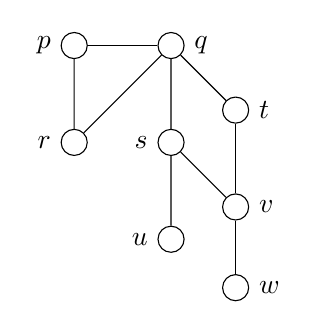
\begin{tikzpicture}[scale=.41]
			    \node[draw,shape=circle, label=left:{$p$}] (AA) at (-8,0) {};
		    	\node[draw,shape=circle, label=right:{$q$}] (AB) at (-5,0) {};
		    	\node[draw,shape=circle, label=left:{$r$}] (AC) at (-8,-3) {};
		    	\node[draw,shape=circle, label=left:{$s$}] (AD) at (-5,-3) {};
		    	\node[draw,shape=circle, label=right:{$t$}] (AE) at (-3,-2) {};
		    	\node[draw,shape=circle, label=left:{$u$}] (AF) at (-5,-6) {};
		    	\node[draw,shape=circle, label=right:{$v$}] (AG) at (-3,-5) {};
		    	\node[draw,shape=circle, label=right:{$w$}] (AH) at (-3,-7.5) {};
		    	
		    	\draw (AA)--(AB);
		    	\draw (AA)--(AC);
		    	\draw (AB)--(AC);
		    	\draw (AB)--(AD);
		    	\draw (AB)--(AE);
		    	\draw (AE)--(AG);
		    	\draw (AD)--(AF);
	    	    \draw (AD)--(AG);
	    	    \draw (AG)--(AH);
		    \end{tikzpicture}
		}
		\subfigure[]{
		    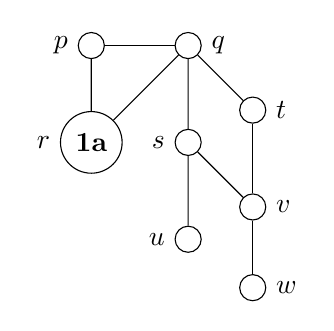
\begin{tikzpicture}[scale=.41]
			    \node[draw,shape=circle, label=left:{$p$}] (AA) at (-8,0) {};
		    	\node[draw,shape=circle, label=right:{$q$}] (AB) at (-5,0) {};
		    	\node[draw,shape=circle, label=left:{$r$}] (AC) at (-8,-3) {\textbf{1a}};
		    	\node[draw,shape=circle, label=left:{$s$}] (AD) at (-5,-3) {};
		    	\node[draw,shape=circle, label=right:{$t$}] (AE) at (-3,-2) {};
		    	\node[draw,shape=circle, label=left:{$u$}] (AF) at (-5,-6) {};
		    	\node[draw,shape=circle, label=right:{$v$}] (AG) at (-3,-5) {};
		    	\node[draw,shape=circle, label=right:{$w$}] (AH) at (-3,-7.5) {};
		    	
		    	\draw (AA)--(AB);
		    	\draw (AA)--(AC);
		    	\draw (AB)--(AC);
		    	\draw (AB)--(AD);
		    	\draw (AB)--(AE);
		    	\draw (AE)--(AG);
		    	\draw (AD)--(AF);
	    	    \draw (AD)--(AG);
	    	    \draw (AG)--(AH);
		    \end{tikzpicture}
		}
		\subfigure[]{
		    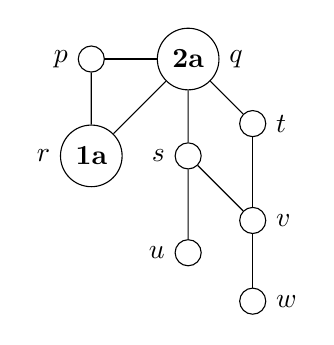
\begin{tikzpicture}[scale=.41]
			    \node[draw,shape=circle, label=left:{$p$}] (AA) at (-8,0) {};
		    	\node[draw,shape=circle, label=right:{$q$}] (AB) at (-5,0) {\textbf{2a}};
		    	\node[draw,shape=circle, label=left:{$r$}] (AC) at (-8,-3) {\textbf{1a}};
		    	\node[draw,shape=circle, label=left:{$s$}] (AD) at (-5,-3) {};
		    	\node[draw,shape=circle, label=right:{$t$}] (AE) at (-3,-2) {};
		    	\node[draw,shape=circle, label=left:{$u$}] (AF) at (-5,-6) {};
		    	\node[draw,shape=circle, label=right:{$v$}] (AG) at (-3,-5) {};
		    	\node[draw,shape=circle, label=right:{$w$}] (AH) at (-3,-7.5) {};
		    	
		    	\draw (AA)--(AB);
		    	\draw (AA)--(AC);
		    	\draw (AB)--(AC);
		    	\draw (AB)--(AD);
		    	\draw (AB)--(AE);
		    	\draw (AE)--(AG);
		    	\draw (AD)--(AF);
	    	    \draw (AD)--(AG);
	    	    \draw (AG)--(AH);
		    \end{tikzpicture}
		}
		\subfigure[]{
		    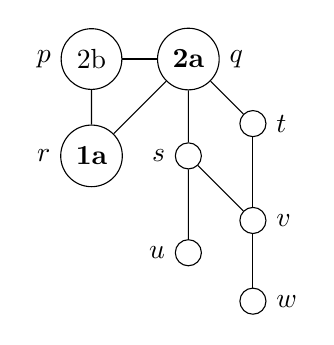
\begin{tikzpicture}[scale=.41]
			    \node[draw,shape=circle, label=left:{$p$}] (AA) at (-8,0) {2b};
		    	\node[draw,shape=circle, label=right:{$q$}] (AB) at (-5,0) {\textbf{2a}};
		    	\node[draw,shape=circle, label=left:{$r$}] (AC) at (-8,-3) {\textbf{1a}};
		    	\node[draw,shape=circle, label=left:{$s$}] (AD) at (-5,-3) {};
		    	\node[draw,shape=circle, label=right:{$t$}] (AE) at (-3,-2) {};
		    	\node[draw,shape=circle, label=left:{$u$}] (AF) at (-5,-6) {};
		    	\node[draw,shape=circle, label=right:{$v$}] (AG) at (-3,-5) {};
		    	\node[draw,shape=circle, label=right:{$w$}] (AH) at (-3,-7.5) {};
		    	
		    	\draw (AA)--(AB);
		    	\draw (AA)--(AC);
		    	\draw (AB)--(AC);
		    	\draw (AB)--(AD);
		    	\draw (AB)--(AE);
		    	\draw (AE)--(AG);
		    	\draw (AD)--(AF);
	    	    \draw (AD)--(AG);
	    	    \draw (AG)--(AH);
		    \end{tikzpicture}
		}
		\subfigure[]{
		    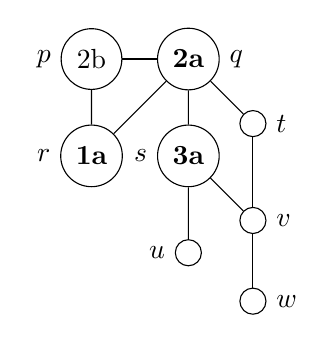
\begin{tikzpicture}[scale=.41]
			    \node[draw,shape=circle, label=left:{$p$}] (AA) at (-8,0) {2b};
		    	\node[draw,shape=circle, label=right:{$q$}] (AB) at (-5,0) {\textbf{2a}};
		    	\node[draw,shape=circle, label=left:{$r$}] (AC) at (-8,-3) {\textbf{1a}};
		    	\node[draw,shape=circle, label=left:{$s$}] (AD) at (-5,-3) {\textbf{3a}};
		    	\node[draw,shape=circle, label=right:{$t$}] (AE) at (-3,-2) {};
		    	\node[draw,shape=circle, label=left:{$u$}] (AF) at (-5,-6) {};
		    	\node[draw,shape=circle, label=right:{$v$}] (AG) at (-3,-5) {};
		    	\node[draw,shape=circle, label=right:{$w$}] (AH) at (-3,-7.5) {};
		    	
		    	\draw (AA)--(AB);
		    	\draw (AA)--(AC);
		    	\draw (AB)--(AC);
		    	\draw (AB)--(AD);
		    	\draw (AB)--(AE);
		    	\draw (AE)--(AG);
		    	\draw (AD)--(AF);
	    	    \draw (AD)--(AG);
	    	    \draw (AG)--(AH);
		    \end{tikzpicture}
		}
		\subfigure[]{
		    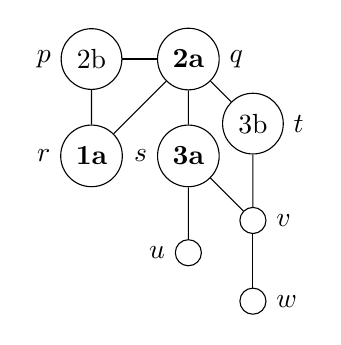
\begin{tikzpicture}[scale=.41]
			    \node[draw,shape=circle, label=left:{$p$}] (AA) at (-8,0) {2b};
		    	\node[draw,shape=circle, label=right:{$q$}] (AB) at (-5,0) {\textbf{2a}};
		    	\node[draw,shape=circle, label=left:{$r$}] (AC) at (-8,-3) {\textbf{1a}};
		    	\node[draw,shape=circle, label=left:{$s$}] (AD) at (-5,-3) {\textbf{3a}};
		    	\node[draw,shape=circle, label=right:{$t$}] (AE) at (-3,-2) {3b};
		    	\node[draw,shape=circle, label=left:{$u$}] (AF) at (-5,-6) {};
		    	\node[draw,shape=circle, label=right:{$v$}] (AG) at (-3,-5) {};
		    	\node[draw,shape=circle, label=right:{$w$}] (AH) at (-3,-7.5) {};
		    	
		    	\draw (AA)--(AB);
		    	\draw (AA)--(AC);
		    	\draw (AB)--(AC);
		    	\draw (AB)--(AD);
		    	\draw (AB)--(AE);
		    	\draw (AE)--(AG);
		    	\draw (AD)--(AF);
	    	    \draw (AD)--(AG);
	    	    \draw (AG)--(AH);
		    \end{tikzpicture}
		}
		\subfigure[]{
		    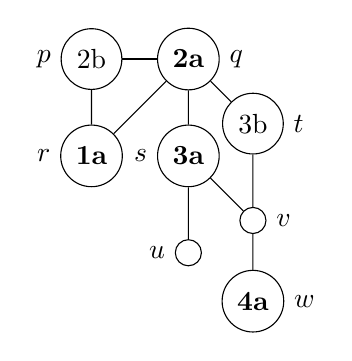
\begin{tikzpicture}[scale=.41]
			    \node[draw,shape=circle, label=left:{$p$}] (AA) at (-8,0) {2b};
		    	\node[draw,shape=circle, label=right:{$q$}] (AB) at (-5,0) {\textbf{2a}};
		    	\node[draw,shape=circle, label=left:{$r$}] (AC) at (-8,-3) {\textbf{1a}};
		    	\node[draw,shape=circle, label=left:{$s$}] (AD) at (-5,-3) {\textbf{3a}};
		    	\node[draw,shape=circle, label=right:{$t$}] (AE) at (-3,-2) {3b};
		    	\node[draw,shape=circle, label=left:{$u$}] (AF) at (-5,-6) {};
		    	\node[draw,shape=circle, label=right:{$v$}] (AG) at (-3,-5) {};
		    	\node[draw,shape=circle, label=right:{$w$}] (AH) at (-3,-7.5) {\textbf{4a}};
		    	
		    	\draw (AA)--(AB);
		    	\draw (AA)--(AC);
		    	\draw (AB)--(AC);
		    	\draw (AB)--(AD);
		    	\draw (AB)--(AE);
		    	\draw (AE)--(AG);
		    	\draw (AD)--(AF);
	    	    \draw (AD)--(AG);
	    	    \draw (AG)--(AH);
		    \end{tikzpicture}
		}
		\subfigure[]{
		    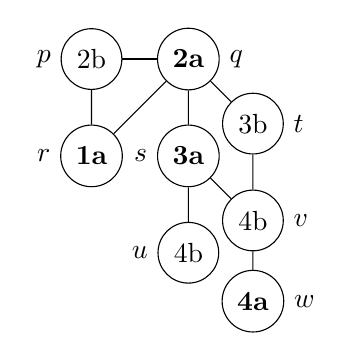
\begin{tikzpicture}[scale=.41]
			    \node[draw,shape=circle, label=left:{$p$}] (AA) at (-8,0) {2b};
		    	\node[draw,shape=circle, label=right:{$q$}] (AB) at (-5,0) {\textbf{2a}};
		    	\node[draw,shape=circle, label=left:{$r$}] (AC) at (-8,-3) {\textbf{1a}};
		    	\node[draw,shape=circle, label=left:{$s$}] (AD) at (-5,-3) {\textbf{3a}};
		    	\node[draw,shape=circle, label=right:{$t$}] (AE) at (-3,-2) {3b};
		    	\node[draw,shape=circle, label=left:{$u$}] (AF) at (-5,-6) {4b};
		    	\node[draw,shape=circle, label=right:{$v$}] (AG) at (-3,-5) {4b};
		    	\node[draw,shape=circle, label=right:{$w$}] (AH) at (-3,-7.5) {\textbf{4a}};
		    	
		    	\draw (AA)--(AB);
		    	\draw (AA)--(AC);
		    	\draw (AB)--(AC);
		    	\draw (AB)--(AD);
		    	\draw (AB)--(AE);
		    	\draw (AE)--(AG);
		    	\draw (AD)--(AF);
	    	    \draw (AD)--(AG);
	    	    \draw (AG)--(AH);
		    \end{tikzpicture}
		    }
	    \caption{Burning a graph. See that part $b$ does not run in step 1 because there is no vertex that was burnt before step 1, so the fire did not spread. Once we label the vertex in some step, we do not change the label in any future steps.}
	    \label{figure:arbitrary-burn-example}
\end{figure}

\begin{definition}\label{definition:burning-sequence}
\textbf{Burning sequence.}\index{burning sequence} The \textit{burning sequence} of
a graph $G$ is the sequence of vertices that were chosen as \textit{fire sources} in part (a) of each time-step to burn a given graph, such that this sequence of vertices is able to burn all the vertices of $G$.
\end{definition}

In the graph demonstrated in \Cref{figure:arbitrary-burn-example}, the burning sequence is $S = (r, q, s, w)$. This means that $r$ was chosen as a fire source in step $1a$, $q$ was chosen as a fire source in step $2a$, and so on.

\section{The underlying problem}\label{section:burn-problem}

Graph burning aims to burn all the vertices in a graph as quickly as possible and has been inspired by other contact processes like firefighting \cite{Hartnell1995}, graph cleaning \cite{Alon2009}, and graph bootstrap percolation \cite{Balogh2012}. The underlying decision problem is described as follows.

\textbf{The decision problem}: Given input is an arbitrary graph $G$ and a constant $k$. The problem is to determine if $G$ can be burnt using a burning sequence of length $k$ or less (or equivalently, in $k$ or less time-steps).\index{graph burning: decision and optimization versions}

Equivalently, we have the optimization version of the graph burning problem.

\textbf{The optimization problem}: Given input is an arbitrary graph $G$. The problem is to compute the minimum number of fire sources (or equivalently, time-steps), that can (collectively in the form of a burning sequence) burn $G$ completely.

With reference to the theory that we established in \Cref{chapter:introduction}, it can be observed that if an optimization algorithm returns a positive integer $k$ as output, the decision algorithm will return $true$ if the input $(G,k)$ is passed to it. Note that the main task in the burning problem is to find a burning sequence of minimum length such that it is able to to burn all the vertices of a graph. Here, we introduce a (new) property of a graph $G$ in \Cref{definition:burning-number}, the \textit{burning number} of a graph $G$ \cite{Bonato2016}, which we denote as $b(G)$.

\begin{definition}\label{definition:burning-number}
\textbf{Burning number.}\index{burning number} The least amount of time steps (or equivalently, fire sources) which are required to burn a graph $G$ is called the \textit{burning number} of $G,\ b(G)$.
\end{definition}

Clearly, the burning number of a graph $G$ tells that how fast $G$ ``can'' be burnt. Observe from \Cref{figure:optimal-burn-example} that the same graph that we burnt in four time-steps in \Cref{figure:arbitrary-burn-example}, can also be burnt in only three time-steps. From \Cref{figure:optimal-burn-example}, we have that the burning sequence $S^{\prime} = (q, v, u)$ of size $3$ is also able to burn this graph completely.

\begin{figure}
	\begin{minipage}{1\textwidth}
		\centering
		    \subfigure[]{
		    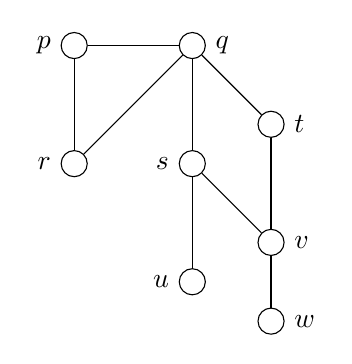
\begin{tikzpicture}[scale=0.5]
		    	\node[draw,shape=circle, label=left:{$p$}] (BA) at (8-8,0) {};
		    	\node[draw,shape=circle, label=right:{$q$}] (BB) at (8-5,0) {};
		    	\node[draw,shape=circle, label=left:{$r$}] (BC) at (8-8,-3) {};
		    	\node[draw,shape=circle, label=left:{$s$}] (BD) at (8-5,-3) {};
		    	\node[draw,shape=circle, label=right:{$t$}] (BE) at (8-3,-2) {};
		    	\node[draw,shape=circle, label=left:{$u$}] (BF) at (8-5,-6) {};
		    	\node[draw,shape=circle, label=right:{$v$}] (BG) at (8-3,-5) {};
		    	\node[draw,shape=circle, label=right:{$w$}] (BH) at (8-3,-7) {};
		    	
		    	\draw (BA)--(BB);
		    	\draw (BA)--(BC);
		    	\draw (BB)--(BC);
		    	\draw (BB)--(BD);
		    	\draw (BB)--(BE);
		    	\draw (BE)--(BG);
		    	\draw (BD)--(BF);
	    	    \draw (BD)--(BG);
	    	    \draw (BG)--(BH);
		    \end{tikzpicture}
		    }
		    \subfigure[]{
		    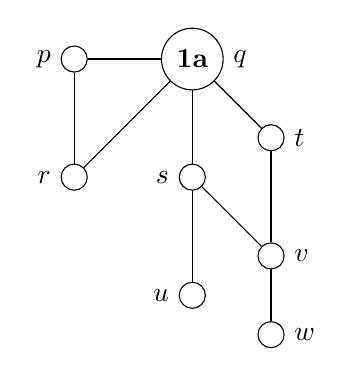
\begin{tikzpicture}[scale=0.5]
		    	\node[draw,shape=circle, label=left:{$p$}] (BA) at (8-8,0) {};
		    	\node[draw,shape=circle, label=right:{$q$}] (BB) at (8-5,0) {\textbf{1a}};
		    	\node[draw,shape=circle, label=left:{$r$}] (BC) at (8-8,-3) {};
		    	\node[draw,shape=circle, label=left:{$s$}] (BD) at (8-5,-3) {};
		    	\node[draw,shape=circle, label=right:{$t$}] (BE) at (8-3,-2) {};
		    	\node[draw,shape=circle, label=left:{$u$}] (BF) at (8-5,-6) {};
		    	\node[draw,shape=circle, label=right:{$v$}] (BG) at (8-3,-5) {};
		    	\node[draw,shape=circle, label=right:{$w$}] (BH) at (8-3,-7) {};
		    	
		    	\draw (BA)--(BB);
		    	\draw (BA)--(BC);
		    	\draw (BB)--(BC);
		    	\draw (BB)--(BD);
		    	\draw (BB)--(BE);
		    	\draw (BE)--(BG);
		    	\draw (BD)--(BF);
	    	    \draw (BD)--(BG);
	    	    \draw (BG)--(BH);
		    \end{tikzpicture}
		    }
		    \subfigure[]{
		    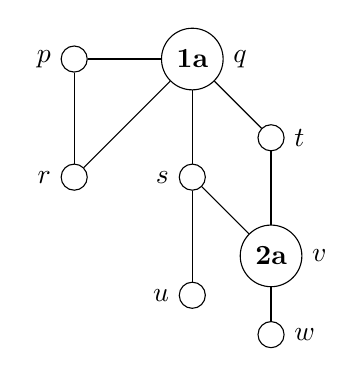
\begin{tikzpicture}[scale=0.5]
		    	\node[draw,shape=circle, label=left:{$p$}] (BA) at (8-8,0) {};
		    	\node[draw,shape=circle, label=right:{$q$}] (BB) at (8-5,0) {\textbf{1a}};
		    	\node[draw,shape=circle, label=left:{$r$}] (BC) at (8-8,-3) {};
		    	\node[draw,shape=circle, label=left:{$s$}] (BD) at (8-5,-3) {};
		    	\node[draw,shape=circle, label=right:{$t$}] (BE) at (8-3,-2) {};
		    	\node[draw,shape=circle, label=left:{$u$}] (BF) at (8-5,-6) {};
		    	\node[draw,shape=circle, label=right:{$v$}] (BG) at (8-3,-5) {\textbf{2a}};
		    	\node[draw,shape=circle, label=right:{$w$}] (BH) at (8-3,-7) {};
		    	
		    	\draw (BA)--(BB);
		    	\draw (BA)--(BC);
		    	\draw (BB)--(BC);
		    	\draw (BB)--(BD);
		    	\draw (BB)--(BE);
		    	\draw (BE)--(BG);
		    	\draw (BD)--(BF);
	    	    \draw (BD)--(BG);
	    	    \draw (BG)--(BH);
		    \end{tikzpicture}
		    }
		    \subfigure[]{
		    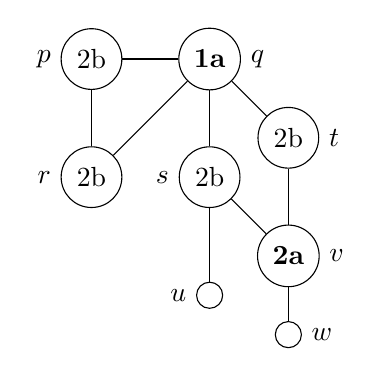
\begin{tikzpicture}[scale=0.5]
		    	\node[draw,shape=circle, label=left:{$p$}] (BA) at (8-8,0) {2b};
		    	\node[draw,shape=circle, label=right:{$q$}] (BB) at (8-5,0) {\textbf{1a}};
		    	\node[draw,shape=circle, label=left:{$r$}] (BC) at (8-8,-3) {2b};
		    	\node[draw,shape=circle, label=left:{$s$}] (BD) at (8-5,-3) {2b};
		    	\node[draw,shape=circle, label=right:{$t$}] (BE) at (8-3,-2) {2b};
		    	\node[draw,shape=circle, label=left:{$u$}] (BF) at (8-5,-6) {};
		    	\node[draw,shape=circle, label=right:{$v$}] (BG) at (8-3,-5) {\textbf{2a}};
		    	\node[draw,shape=circle, label=right:{$w$}] (BH) at (8-3,-7) {};
		    	
		    	\draw (BA)--(BB);
		    	\draw (BA)--(BC);
		    	\draw (BB)--(BC);
		    	\draw (BB)--(BD);
		    	\draw (BB)--(BE);
		    	\draw (BE)--(BG);
		    	\draw (BD)--(BF);
	    	    \draw (BD)--(BG);
	    	    \draw (BG)--(BH);
		    \end{tikzpicture}
		    }
		    \subfigure[]{
		    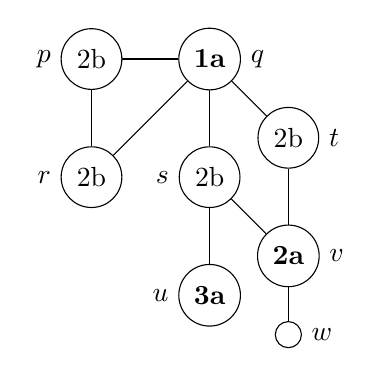
\begin{tikzpicture}[scale=0.5]
		    	\node[draw,shape=circle, label=left:{$p$}] (BA) at (8-8,0) {2b};
		    	\node[draw,shape=circle, label=right:{$q$}] (BB) at (8-5,0) {\textbf{1a}};
		    	\node[draw,shape=circle, label=left:{$r$}] (BC) at (8-8,-3) {2b};
		    	\node[draw,shape=circle, label=left:{$s$}] (BD) at (8-5,-3) {2b};
		    	\node[draw,shape=circle, label=right:{$t$}] (BE) at (8-3,-2) {2b};
		    	\node[draw,shape=circle, label=left:{$u$}] (BF) at (8-5,-6) {\textbf{3a}};
		    	\node[draw,shape=circle, label=right:{$v$}] (BG) at (8-3,-5) {\textbf{2a}};
		    	\node[draw,shape=circle, label=right:{$w$}] (BH) at (8-3,-7) {};
		    	
		    	\draw (BA)--(BB);
		    	\draw (BA)--(BC);
		    	\draw (BB)--(BC);
		    	\draw (BB)--(BD);
		    	\draw (BB)--(BE);
		    	\draw (BE)--(BG);
		    	\draw (BD)--(BF);
	    	    \draw (BD)--(BG);
	    	    \draw (BG)--(BH);
		    \end{tikzpicture}
		    }
		    \subfigure[]{
		    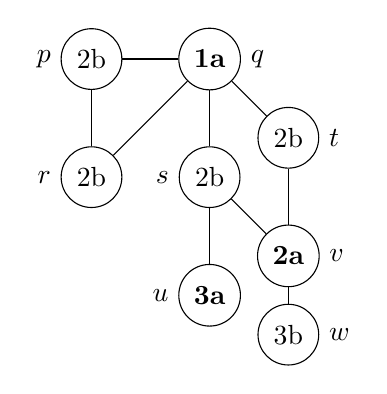
\begin{tikzpicture}[scale=0.5]
		    	\node[draw,shape=circle, label=left:{$p$}] (BA) at (8-8,0) {2b};
		    	\node[draw,shape=circle, label=right:{$q$}] (BB) at (8-5,0) {\textbf{1a}};
		    	\node[draw,shape=circle, label=left:{$r$}] (BC) at (8-8,-3) {2b};
		    	\node[draw,shape=circle, label=left:{$s$}] (BD) at (8-5,-3) {2b};
		    	\node[draw,shape=circle, label=right:{$t$}] (BE) at (8-3,-2) {2b};
		    	\node[draw,shape=circle, label=left:{$u$}] (BF) at (8-5,-6) {\textbf{3a}};
		    	\node[draw,shape=circle, label=right:{$v$}] (BG) at (8-3,-5) {\textbf{2a}};
		    	\node[draw,shape=circle, label=right:{$w$}] (BH) at (8-3,-7) {3b};
		    	
		    	\draw (BA)--(BB);
		    	\draw (BA)--(BC);
		    	\draw (BB)--(BC);
		    	\draw (BB)--(BD);
		    	\draw (BB)--(BE);
		    	\draw (BE)--(BG);
		    	\draw (BD)--(BF);
	    	    \draw (BD)--(BG);
	    	    \draw (BG)--(BH);
		    \end{tikzpicture}
		}
	    \end{minipage}
	    \caption{(Better) Burning procedure (optimal) on an example graph. The subject graph is same as that on which an arbitrary burning procedure is demonstrated in \Cref{figure:arbitrary-burn-example}.}
	    \label{figure:optimal-burn-example}
    \end{figure}

Observe that the example graph, on which two different burning procedures are demonstrated, in \Cref{figure:arbitrary-burn-example} and \Cref{figure:optimal-burn-example} respectively, requires at least $3$ time steps to be burnt; it cannot be burned in less than $3$ time steps. So $S^{\prime}$ is an optimal burning sequence which can burn this graph. Burning number of this graph is $3$.

Let that a burning procedure burns a graph in $k$ time steps. While burning a graph, it is noticeable that if at a step $i$ a vertex $v \in G$ is chosen as a fire source, then at each subsequent step, the set of vertices to which $v$ spreads fire to keeps on increasing till the $k^{th}$ step: at a time step $i+t$, $v$ is able to burn all the vertices in $G.N_t[v]$. Here, we define the \textit{burning cluster} of a fire source in \Cref{definition:burning-cluster} as follows.

\begin{definition}\label{definition:burning-cluster}
\textbf{Burning cluster.}\index{burning cluster} Let that a burning sequence $S=(x_1,x_2,\dots,x_k)$ of size $k$ is able to burn a graph $G$. The burning cluster of a fire source $x_i$ (the fire source chosen at the time-step $i$) is the set of vertices to which $x_i$ is able to spread fire till the end of the burning process (till the $k^{th}$ time-step). This set contains all the vertices in $G.N_{k-i}[x_i]$.
\end{definition}

If $S = (x_1, x_2, x_3, . . ., x_k)$ is the burning sequence which is capable of burning $G$, \Cref{equation:burn-verify} \cite{Bessy2017} must follow.

\begin{equation}\label{equation:burn-verify}
    G.N_{k-1}[x_1] \cup G.N_{k-2}[x_2] \cup . . . \cup G.N_0[x_k] = G.V.
\end{equation}

\section{Reviewing graph burning theory}\label{section:burning-literature}

The burning number was introduced in \cite{Bonato2016}. This work showed that the burning number of a path or cycle of length $n$ is $\lceil\sqrt{n}\rceil$. They have presented some other properties and results also related to the graph burning problem. Bessy et al. \cite{Bessy2017} showed that general graph burning is NP-Complete. They showed that optimal burning spider graphs, trees, and path-forests is NP-Complete. A 3-approximation algorithm for burning general graphs was described in \cite{Bessy2017}. Bonato et al. \cite{Bonato2019} proposed a $2$-approximation algorithm for burning trees. A 2-approximation algorithm for graphs bounded by a diameter of constant length was described in \cite{Kamali2019,Kamali2020}. A 1.5 approximation algorithm for burning path forests was described in \cite{Bonato2019a}. This article also showed that burning number of spider graphs of order $n$ is atmost $\sqrt{n}$. Simon et al. \cite{Simon2019} presented systems that utilize burning in the spread of an alarm through a network.
Bessy et al. \cite{Bessy2018} proved that the burning number of a connected graph of order $n$ is at most $\sqrt{\frac{12n}{7}}+3 \approx 1.309\sqrt{n}+3$. They also showed that the burning number of trees with $n_2$ vertices of degree $2$, and $n (\geq3)$ vertices of degree at least $3$ is at most $\sqrt{(n+n_2)+\frac{1}{4}}+\frac{1}{2}$. \cite{Simon2019a} have provided heuristics to minimize the time steps in burning a graph. They have studied that which vertices should be selected to be burnt from ``outside'' and in which time-steps.

\section{Verification of a burning sequence}\label{section:burning-verify}

As discussed in \Cref{section:problems-classes}, a problem which can be verified deterministically in polynomial time is in NP class. We can verify the validity of a burning sequence in polynomial time. Every burning sequence which satisfies \Cref{equation:burn-verify} is is able to burn $G$ completely, but apart from this, here we also verify that no fire source in a burning sequence should be placed on the vertex which has already been burnt. \Cref{algorithm:burn-verify}\index{burning sequence - verifying correctness} verifies if a given burning sequence $S$ is a valid burning sequence for a graph $G$.

\begin{algorithm}\label{algorithm:burn-verify}
Given an input graph $G$ and a burning sequence $S = (x_1, x_2, x_3, . . ., x_k)$ of length $k$, perform the following steps.
\end{algorithm}

\textbf{\textit{Stage 1.}} If $S$ does not satisfy \Cref{equation:burn-verify}, then return $false$.

\textbf{\textit{Stage 2.}} $\forall\ 1\leq i\leq k-1$, perform the following steps.

\textbf{\textit{Stage 2.1.}} $\forall\ i+1\leq j\leq k$, if $x_j \in G.N_{j-i-1}[x_i]$, then return $false$.

\textbf{\textit{Stage 3.}} Return $true$.\\

If \Cref{algorithm:burn-verify} returns $true$ for the input $(G,S)$, it means that $S$ is a valid burning sequence and is able to burn $G$ completely. \Cref{algorithm:burn-verify} can be implemented in $O(n^2)$ time. This also implies that the graph burning problem is in NP. We state the formally in \Cref{lemma:burning-in-NP}. In fact, optimal burning of general graphs is NP-Hard. We discuss this in the following chapters in detail.

\begin{lemma}\label{lemma:burning-in-NP}
    The (optimal) graph burning problem is in NP.
\end{lemma}

\section{Related problems and games}\label{section:related-games}

As discussed in \Cref{section:burn-problem}, the procedures of certain other problems such as firefighter problem, graph cleaning and graph bootstrap percolation are similar to the procedure of the graph burning problem. In the following few paragraphs in this section, we shall discuss them in brief.

\subsection{Firefighter problem}

The aim of the \textit{firefighter}\index{firefighter problem} problem \cite{Fomin2016} is to save as many vertices of a given graph $G$ as possible from a fire that starts from a single vertex. At step $1$, an arbitrary vertex is burned. At each step $t$, $t \geq 2$, first (a) a firefighter can be placed on an unburned vertex and this firefighter protects that node from fire till the last time-step, and then (b) the fire spreads to the unprotected vertices adjacent to the vertices which are burned till step $t-1$. This process continues till fire cannot spread to any more vertices.

The input is the subject graph $G$ and one fire source $s$. The task is to save the maximum possible number of vertices from fire.

\subsection{Firefighter reserve problem}

\textit{Firefighter reserve deployment}\index{firefighter reserve deployment problem} \cite{Fomin2016} problem proceeds as follows. The fire gets initiated from a single fire source. Initially, there is one firefighter in the firefighter reserve. In each step $t, t \geq 2$, (a) some or no firefighters (subject to availability in the firefighter reserve) are placed, each on an unburned vertex, (b) the fire spreads from the burned vertices to their adjacent vertices which are not protected (by a firefighter), (c) one firefighter increases in the firefighter reserve. This process continues until fire can spread no further.

\subsection{Graph cleaning}

In the \textit{graph cleaning}\index{cleaning: graph} problem, at the beginning, all the vertices and the edges are considered ``dirty''. There are a fixed number of available cleaning brushes. At each step, one vertex $v$ and all the edges incident to $v$ which are dirty may be cleaned if the number of brushes on $v$ are equal to the dirty edges incident on $v$. No brush cleans any edge which is already clean. If a brush cleans an edge, the edge is considered to be traversed. A vertex is cleaned if all the edges incident to it are cleaned, and the cleaning process is done on a vertex $v$ only if we can clean each edge incident on it. A graph $G$ is considered cleaned when each vertex of $G$ has been cleaned. Graph cleaning was introduced in \cite{Mckeil2007,Messinger2008}.

The input is an arbitrary graph $G$, and a constant $k$ number of brushes. The task is to determine if $G$ can be cleaned by $k$ brushes. Equivalently, the optimization problem can be to compute the minimum number of brushes that are required to clean an arbitrary graph.

\subsection{Graph bootstrap percolation}

A phenomenon in graphs called \textit{weak saturation}\index{bootstrap percolation: graph} was introduced by Bollobas in 1968. Given a graph $H$, another graph $G$ of $n$ vertices is called \textit{weakly $H$-saturated} if no subgraph of $G$ can make $H$, but $\exists$ a non-empty set $A$ consisting of edges missing in $G$ such that $\forall\ e \in A$, $H$ is a subgraph of $G+e$ \cite{Faudree2013,Balogh2012,Bollobas2017}. \cite{Balogh2012} observed that weak saturation is strongly related to bootstrap percolation, which was introduced in \cite{Chalupa1979}. \nocite{Faudree2013}

In \textit{bootstrap percolation}, the inputs are an arbitrary graph $G$ and an infection threshold $r>2$. We choose a set of initially ``infected'' vertices $A \subseteq G.V$; we declare the remaining vertices $G.V \setminus A$ ``healthy''.

Then, in consecutive time steps, we infect all healthy vertices which have at least $r$ infected neighbours.  We say that $A$ percolates if, starting from $A$ we are able to finally infect every vertex in $G.V$. More precisely, we set $A_0=A$ and for $t= 1,2,3,...$, we compute $A_t$ according to \Cref{equation:bootstrap-percolation} \cite{Faudree2013} as follows.

\begin{equation}\label{equation:bootstrap-percolation}
    A_t = A_{t-1} \cup \{v\in V: | G.N[v]\cap A_{t-1}| \geq r\}
\end{equation}

Hence $A$ percolates if after computing on equation \thech.2 indefinitely, we infect all the vertices, that is, $\mathop{\cup}_{t=0}^\infty A_t = G.V$.

\section{Overview of possible applications}

Burning a graph can be used to model the spread of a meme, social gossip, emotion, or a social contagion. It can also be used to model spread of viral infections, or otherwise the exposure to infections and proliferation of virus in the body.
Graph burning is relatively a newly introduced procedure. Currently, not much works have come in public domain which utilize the graph burning in modelling of practically applicable systems.

{\~S}imon et al. \cite{Simon2019} have provided heuristics for usage in for spreading an alarm or other critical information in minimum amount of time steps. This may include spread of information via satellite, or throughout a terrestrial network, for example.
They have assumed that a satellite can spread information only sequentially: to one target node (person, device, etc) at a time. On the other hand, each node in their system is able to spread the information parallelly through the available technologies.

Simon et al. \cite{Simon2019a} have simulated a network which tries to spread alarms to all the nodes in the least amount of time steps. The nodes are connected to each other, and at the start of each time step, a new node is alarmed from ``outside''. Also during each time step, the alarmed nodes alarm their neighbour nodes, same as the graph burning procedure. This process stops when all the nodes are alarmed.

\section{Computational limitations}

Optimal graph burning is hard \cite{Bessy2017} for general graphs, like several other problems such as coloring a graph, finding the largest clique in a graph, or finding maximum sized independent set of a graph. It has been shown that graph burning is NP-Complete for several graph classes, even when computing other properties, which are NP-Hard for general graph classes, is ``easy'': graph classes on which other NP-Hard problems can be solved in polynomial time. It has been proved in \cite{Bessy2017} that burning a spider graph, path forests, and trees with maximum degree 3 is NP-Complete.

On the other hand, we have a 3-approximation algorithm for burning general graphs, a 2-approximation algorithm for burning trees, a 2-approximation algorithm for burning the graphs bounded by a diameter of constant length, and a 1.5-approximation algorithm for burning path forests, as discussed in \Cref{section:burning-literature}.

In the following chapters, we discuss these characteristics of the graph burning problem in detail from the perspective of certain graph classes. For the overview of chapters, see \Cref{section:organization-of-chapters}.

% \bibliography{ref.bib}
% \bibliographystyle{plain}